The main results from \cite{main} which we are exploring in this paper deal with a special type of space called a \textit{Banach space} --- recall we very briefly mentioned Banach spaces at the end of section 2.1.  More specifically, a special subset of Banach spaces, called $l^p$ spaces, are used extensively in \cite{main}.

\begin{defn}
A metric space $(X,d)$ is called \textbf{complete} if every Cauchy sequence in $X$ converges to some in $E$.
\end{defn}

\begin{defn}
A normed vector space $(V, ||\cdot||)$ is called a \textbf{Banach space} if and only if $V$ is complete in the metric induced from the norm.
\end{defn}

Our first example of a Banach space requires a result known as the Bolzano-Weierstrass theorem to prove completeness.

\begin{theorem}[Bolzano-Weierstrass]
Every bounded sequence has a convergent subsequence.
\end{theorem}

\begin{proof}
Suppose $(s_n)$ is a bounded sequence.  By Theorem 2.14, $(s_n)$ has a monotonic subsequence, $(s_{n_k})$.  Since $(s_n)$ is a bounded sequence, $(s_{n_k})$ is bounded as well.  Since all bounded monotonic subsequences converge, we have that $(s_{n_k})$ converges.
\end{proof}

We now have all the necessary tools in order to easily show certain spaces are complete.

\begin{example}
Consider the normed vector spaces $\mathbb{Q}, \mathbb{R}, \mathbb{C}$.
\begin{itemize}
\item $\mathbb{R}$ with the standard Euclidean norm is a Banach space \cite{nthubanach}. 

We already know that $\mathbb{R}$ is a normed vector space.  So to prove it is a Banach space, we must show it is complete.  That is, we must show that every Cauchy sequence in $\mathbb{R}$ converges to a point in $\mathbb{R}$.  This follows immediately from three previous theorems.  First, note every Cauchy sequence is bounded (Theorem 2.17).  By Bolzano-Weierstrass, every bounded sequence in $\mathbb{R}$ has a convergent subsequence (with limit in $\mathbb{R}$).  Finally, if a subsequence of a Cauchy sequence converges, then the whole sequence converges to the same point (Theorem 2.19).  Thus $\mathbb{R}$ is complete, and is hence a Banach space.

\item $\mathbb{C}$ with its standard norm is a Banach space.  Indeed, if $(z_n) = (x_n) + i(y_n)$ is Cauchy in $\mathbb{C}$, then $(x_n)$ and $(y_n)$ are Cauchy in $\mathbb{R}$.  Since $\mathbb{R}$ is complete, we have $(x_n)$ converges to $x$ and $(y_n)$ converges to $y$, $x, y \in \mathbb{R}$.  Thus we have that $(z_n)$ converges to $z = x + iy$.  Hence $\mathbb{C}$ is complete and is thus a Banach space.

\item The metric space $(\mathbb{Q}, d)$ with its usual metric is not complete.  This is because there are Cauchy sequences in $\mathbb{Q}$ which converge to irrational limits.  For example, 
\[(s_n) = \biggl ( 1 + \frac{1}{n} \biggr )^n\]
is contained in $\mathbb{Q}$, but converges to $e$ which is not in $\mathbb{Q}$.
\end{itemize}
\end{example}

The following lemma is often useful in proving that a metric space is complete.

\begin{lemma}
Let $(X,d)$ be a metric space.  If every Cauchy sequence has a convergent subsequence in $X$, then $(X,d)$ is complete.
\end{lemma}

Now we will provide a criterion for completion of a normed space in terms of series.

\begin{defn}
There are a number of terms we must define for series.
\begin{itemize}
\item If $(E, ||\cdot||)$ is a normed space then a \textbf{series} in $E$ is just the summation a sequence $(x_n)$ of terms $x_n \in E$ denoted \[\sum_{k=m}^{n}x_n;\]
\item The sum 
\[s_n = \sum_{k=m}^{n}x_n\]
is called the \textbf{nth partial sum} of the series;
\item The series \textbf{converges} if the sequence of partial sums has a limit.  That is, if there exists $s \in E$ such that
\[\lim_{n \to \infty} \biggl|\biggl|\biggl(\sum_{k=m}^{n}x_k\biggr) - s\biggr|\biggr| = 0.\]
If the sequence of partial sums has no limit in $E$, we say the series \textbf{diverges};
\item We say a series $\sum_{n=m}^\infty x_n$ is \textbf{absolutely convergent} if $\sum_{n=m}^\infty ||x_n|| < \infty$.  This is because $\sum_{n=m}^\infty ||x_n||$ is the summation of a series of real positive terms, so the sequence of partial sums either converges in $\mathbb{R}$ or increases to $\infty$.
\end{itemize}
\end{defn}

\begin{defn}
A series satisfies the \textbf{Cauchy criterion} if its sequence of partial sums forms a Cauchy sequence.
\end{defn}

\begin{theorem}[Series criterion for completion]
Let $(E, ||\cdot||)$ be a normed vector space.  $E$ is complete (and thus is a Banach space) if and only if each absolutely convergent series $\sum_{n=1}^\infty x_n$ of terms $x_n \in E$ is convergent in $E$.
\end{theorem}

\begin{proof}
We begin with the forward direction.  Suppose $E$ is complete and $\sum_{n=q1}^{n}||x_j|| < \infty$.  Then the individual partial sums of this series
\[S_n = \sum_{j=1}^{n}||x_j||\]
must satisfy Cauchy criterion.  That is, for any $\epsilon > 0$, there exists $N$ such that if $n, m \geq N$, then $|S_n - S_m| < \epsilon$.  So suppose $n > m \geq N$.  Then,
\[|S_n - S_m| = \biggl|\sum_{j=1}^{n} ||x_j|| - \sum_{j=1}^{m} ||x_j||\biggr| = \sum_{j = m+1}^{n} ||x_j|| < \epsilon.\]
Now, consider the partial sums $s_n = \sum_{j=1}^{n} x_j$.  If $n>m\geq N$, then
\[||s_n - s_m|| = \biggl|\biggl|\sum_{j=1}^{n} x_j - \sum_{j=1}^{m} x_j\biggr|\biggr| = \biggl|\biggl|\sum_{j = m+1}^{n} x_j\biggr|\biggr| \leq \sum_{j=m+1}^{n} ||x_j|| < \epsilon.\]
Hence the sequence $(s_n)$ is Cauchy in $E$.  Since $E$ is complete, $\lim_{n \to \infty} s_n$ exists in $E$, and so $\sum_{n=1}^{\infty} x_n$ converges.  This completes the forward direction.

For the other direction, assume all absolutely convergent series in $E$ are convergent.  Let $(u_n)$ be a Cauchy sequence in $E$.  Then we can find $n_1 > 0$ such that if $n,m \geq n_1$ then 
\[||u_n - u_m|| < \frac{1}{2}.\]
We can also find $n_2 > 1$ such that if $n,m > n_2$ then
\[||u_n - u_m|| < \frac{1}{4} = \frac{1}{2^2}.\]
Without loss of generality we can assume that $n_2 > n_1$.  By continuing to pick $n_j$ in this way, we can find $n_1 < n_2 < n_3 < \cdots$ such that if $n,m \geq n_j$ then
\[||u_n - u_m|| < \frac{1}{2^j}.\]
Now, consider the series $\sum_{j=1}^{\infty}x_j = \sum_{j=1}^{\infty}(u_{n_{j+1}} - u_{n_j})$ (Note this is a subseries of $(u_n)$.  Then,
\begin{align*}
\sum_{j=1}^{\infty}||x_j|| &= \sum_{j=1}^{\infty}||u_{n_{j+1}} - u_{n_j}||\\
&\leq \sum_{j=1}^{\infty} \frac{1}{2^j}\\
&= 1 < \infty.
\end{align*}
Thus $\sum_{j=1}^{\infty}x_j$ is absolutely convergent and, by our assumption, must also be convergent.  Thus its sequence of partial sums
\[s_J = \sum_{j=1}^{J}(u_{n_{j+1}} - u_{n_j}) = u_{n_{J+1}} - u_{n_1}\]
has a limit in $E$.  Thus,
\[\lim_{J \to \infty} u_{N_{J+1}} = u_{n_1} + \lim_{J \to \infty} (u_{N_{J+1}} - u_{n_1})\]
exists in $E$.  We have shown that $(u_n)$ has a convergent subsequence in $E$.  By Lemma 4.4, we finally have that $E$ is complete.
\end{proof}

We now look at a special family of Banach spaces known as $l^p$-spaces.  $l^p$-spaces are the main type of space we will be working in in the main results section of the paper.

\begin{defn}
For $1 \leq p < \infty$, $l^p$ denotes the set of all sequences $x = \{a_n\}_{n=1}^{\infty}$ which satisfy
\[\sum_{n=1}^{\infty} |a_n|^p < \infty.\]
If $p = \infty$, we define $p^{\infty}$ as the set of all sequences $x = \{a_n\}_{n=1}^{\infty}$ which satisfy
\[\sup_{n \geq 1} |a_n| < \infty\]
\end{defn}

In other words, for $1 \leq p < \infty$, $l^p$ is the set of all sequences whose series converge when each of its individual elements is raised to the $p^{\textrm{th}}$ power.  $l^{\infty}$ is the set of all sequences whose limit is not infinity --- that is, the set of all bounded sequences.  We commonly combine $l^p$ with the following norms, called the \textit{$p$-norms}:

For $x = (a_n) \in l^p$, define
\[||x||_p = \biggl(\sum_{n=1}^{\infty}|a_n|^p\biggr)^{1/p}, \;\; \textrm{ for } p < \infty;\]
\[||x||_{\infty} = \sup_{n \geq 1} |a_n|.\]

It is very easy to see that the $l^p$ spaces are nested; as $p$ increases, $l^p$ become more permissive.  That is, 
\[l^1 \subset l^2 \subset l^3 \subset \cdots \subset l^{\infty}.\]

\begin{example}
We demonstrate the nesting of $l^p$.
Consider the harmonic sequence $(s_n) = \frac{1}{n}$.  It is well known that
\[\sum_{n=1}^{\infty} \biggl|\frac{1}{n}\biggr| = \infty.\]
Thus $(s_n) \notin l^1$.\\
However, 
\[\sum_{n=1}^{\infty} \biggl|\frac{1}{n}\biggr|^2 = \sum_{n=1}^{\infty} \biggl|\frac{1}{n^2}\biggr| < \infty.\]
Thus $(s_n) \in l^2$.  Similarly, $(s_n) \in l^p$ for $p > 2$.
\end{example}

We can also easily see that the $p$-norms are nested as well.  We show this by drawing the unit ball
\[\{x \in \mathbb{R}^2 : ||x||_p \leq 1\}\]
for each $p$-norm in $\mathbb{R}^2$ (Figure 3).

\begin{figure}[h]
\centering
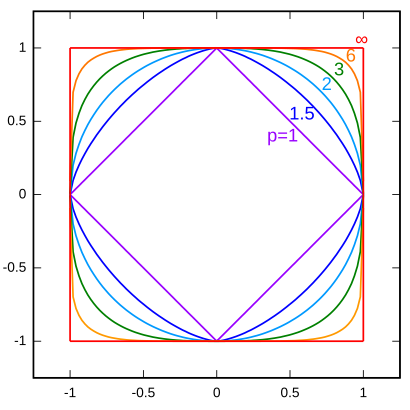
\includegraphics[scale=0.5]{images/p-norms.png}
\caption{The unit ball of various $p$-norms \cite{pnormpic}}
\end{figure}

We now show that $l^p$ is a Banach space under its appropriate p-norm.  We do this in several steps, first showing $l^p$ is a vector space.  Then, we prove the properties of a norm hold for the p-norms.  Finally, we show that $l^p$ is complete.  Note we often omit the cases for $p=1$ and $p=\infty$, as those cases will sometimes require separate arguments which are simple and direct.

\begin{prop}
$l^p (1 \leq p \leq \infty)$ is a vector space.
\end{prop}

\begin{proof}
If $x \in l^p$ and $c \in \mathbb{C}$, then clearly $cx \in l^p$.  Then, if $x,y \in l^p$, since $|x_n + y_n| \leq (2|x_n|^p) + (2|y_n|^p)$, we also have that $x+y \in l^p$.  So addition and scalar multiplication can be defined on $l^p$.  Now, algebraic operations on $l^p$ are defined componentwise; for example, $x+y$ is the sequence whose $n$th element is $x_n + y_n$.  Since all operations are defined this way, the algebraic rules for $l^p$ are simply inherited from $\mathbb{C}$.
\end{proof}

\begin{prop}
$||\cdot||_p$ is a norm on $l^p$
\end{prop}

The first two properties of a norm are obvious.  To prove the triangle inequality, though, we must first prove an inequality known as H{\"o}lder's inequality.  For H{\"o}lder's inequality, we need the following Lemma, which we will take as given.

\begin{lemma}
Suppose $1 < p < \infty$ and q is defined by $\frac{1}{p} + \frac{1}{q} = 1$.  Then,
\[ab \leq \frac{a^p}{p} + \frac{b^q}{q} \qquad \textrm{ for } a,b \geq 0.\]
\end{lemma}

\begin{example}[of previous Lemma]
Suppose $p = 3$.  Then $q = \frac{3}{2}$ since $\frac{1}{p} + \frac{1}{q} = 1$.  Consider several values for $a$ and $b$.
\begin{itemize}
\item $a = 1, b=1$\\
$(1)(1) = 1.$  $\frac{1^3}{3} + \frac{1^{3/2}}{3/2} = \frac{1}{3} + \frac{2}{3} = 1$ 
\item $a = 4, b=9$\\
$(4)(9) = 36$.  $\frac{4^3}{3} + \frac{9^{3/2}}{3/2} = \frac{64}{3} + \frac{54}{3} = \frac{118}{3} > 36$.
\item $a = 20, b=64$\\
$(20)(64) = 1280$.  $\frac{20^3}{3} + \frac{64^{3/2}}{3/2} = \frac{8000}{3} + \frac{1024}{3} = \frac{9024}{3} = 3008$.
\end{itemize}
\end{example}

\begin{lemma}[H{\"o}lder's Inequality]
Let $x \in l^p, y \in l^q,$ where $1 \leq p < \infty$ and
$\frac{1}{p} + \frac{1}{q} = 1.$
Then,
\[||xy||_1 = \sum_{n=1}^{\infty} |a_nb_n| \leq ||(a_n)_n||_p||(b_n)_n||_q.\]
\end{lemma}

This inequality also shows that $xy \in l^1$ under the same conditions.  Note that if $p=1$, we interpret this to mean that $q = \infty$.

\begin{proof}
If $p=1$ and $q= \infty$, this is obvious.  So, suppose $p > 1$.  Let $A$ and $B$ be as follows:
\begin{align*}
A \; &= \; ||x||_p = \biggl(\sum_{n=1}^{\infty} |a_n|^p\biggr)^{1/p}\\
B \; &= \; ||y||_q = \biggl(\sum_{n=1}^{\infty} |b_n|^q\biggr)^{1/q}
\end{align*}
If either $A=0$ or $B=0$, the inequality is obviously true; both sides must equal 0.  So, assume $A \neq 0, B\neq 0$ and use Lemma 4.13 with $a = |a_n|/A$ and $b = |b_n|/B$ to see
\begin{align*}
\frac{|a_nb_n|}{AB} &\leq \frac{1}{p}\frac{|a_n|^p}{A^p} + \frac{1}{q}\frac{|b_n|^1}{B^q}\\
\textrm{So } \sum_{n=1}^{\infty} \frac{|a_nb_n}{AB} &\leq \frac{1}{p}\sum_{n=1}^{\infty}\frac{|a_n|^p}{A^p} + \frac{1}{q}\sum_{n=1}^{\infty}\frac{|b_n|^1}{B^q}\\
&= \frac{1}{p} + \frac{1}{q}\\
&= 1.
\end{align*}
Hence
\[\sum_{n=1}^{\infty}|a_nb_n| \leq AB = ||x||_p||y||_q.\]
\end{proof}

\begin{lemma}[Minkowski's inequality or triangle inequality for $l^p$]
If $x,y \in l^p (1 \leq p \leq \infty)$, then $x+y \in l^p$ and
\[||x+y||_p \leq ||x||_p + ||y||_p\]
\end{lemma}

\begin{proof}
This inequality is trivial for $p=1$ and $p=\infty$, so suppose $1 < p < \infty$.  We already know $(x_n + y_n)_n \in l^p$ (Proposition 4.11).  For the inequality, observe that
\begin{align*}
\sum_n |x_n + y_n|^p &= \sum_n |x_n + y_n|\,|x_n + y_n|^{p-1}\\
&= \sum_n |x_n|\,|x_n + y_n|^{p-1} + \sum_n |y_n|\,|x_n + y_n|^{p-1}.
\end{align*}
Let $(a_n) = |x_n|$ and $(b_n) = |x_n + y_n|^{p-1}$.  So $(a_n) \in l^p$.  Also, $(b_n) \in l^p$ since
\begin{align*}
\sum_n (b_n)^q &= \sum_n |x_n + y_n|^{(p-1)q}\\
&= \sum_n |x_n + y_n|^p \qquad\textrm{ since } \frac{1}{p} + \frac{1}{q} = 1\\
&< \infty \qquad\textrm{ since we know } (x_n + y_n)_n \in l^p.\\
\end{align*}
Now, from H{\"o}lder's inequality, we have
\begin{align*}
\sum_n |x_n|\,|x_n+y_n|^{p-1} &\leq \biggl(\sum_n |x_n|^p\biggr)^{1/p} \biggl(\sum_n |x_n + y_n|^{(p-1)q}\biggr)^{1/q}\\
&= (||x||_p\,||x + y||_p)^{p/q}
\end{align*}
Similarly, we have
\[\sum_n|x_n|\,|x_n + y_n|^{p-1} \leq ||y||_p\bigl(||x+y||_p\bigr)^{p/q}.\]

If we add the two inequalities, we are left with
\[\bigl(||x+y||_p\bigr)^p \leq ||x||_p\bigl(||x + y||_p\bigr)^{p/q} + ||y||_p\bigl(||x+y||_p\bigr)^{p/q}.\]

Now, if $||x+y||_p = 0$, then Minkowski's inequality is true since a property of norms is that $||\cdot|| \geq 0$.  So suppose $||x+y||_p \neq 0$.  Then we can divide both sides of the inequality by $\bigl(||x+y||_p\bigr)^{p/q}$ to get
\[\bigl(||x+y||_p\bigr)^{p-p/q} \leq ||x||_p + ||y||_p.\]
Since, $p-\frac{p}{q} = 1$, we have achieved our goal.
\end{proof}

At this point, we have that $l^p$ is a normed vector space for $1 \leq p \leq \infty$.  To show that $l^p$ is a Banach space, all that remains is to show that $l^p$ is complete.  The proof of this requires some awkward notation, since the elements of $l^p$ are sequences themselves --- so, a sequence of elements in $l^p$ is a sequence of sequences.  So in a sequence of sequences in $l^p$, we will use a superscript to denote the $n$th sequence --- i.e. $x^{(n)}$ is the $n$th sequence.

\begin{theorem}
$l^p$ is a complete under the norm
\[||x||_p = \biggl(\sum_{n=1}^{\infty}|x_n|^p\biggr)^{1/p}\]
for $x \in l^p, 1 < p < \infty$.
\end{theorem}

\begin{proof}
Suppose $x^{(n)} \in l^p$ be a Cauchy sequence.  Let $\epsilon > 0$.  Since $x^{(n)}$ is Cauchy, there exists $n_0 \in \mathbb{N}$ such that if $n,m > n_0$, then
\[\sum_{j=1}^{\infty} |x_j^{(n)} - x_j^{(m)}|^p < \epsilon ^p.\]
So, for each fixed $j \in \mathbb{N}$,
\[|x_j^{(n)} - x_j^{(m)}| \leq \biggl(\sum_{j=1}^{\infty} |x_j^{(n)} - x_j^{(m)}|^p\biggr)^{1/p} < \epsilon .\]
That is, $(x_j^{(n)})$ is a Cauchy sequence in $\mathbb{C}$.  Since $\mathbb{C}$ is complete, these sequences have limits in $\mathbb{C}$.  Define
\[x_j = \lim_{n \to \infty} x_j^{(n)}.\]
Let $x = (x_j)$.  So, we have $x^{(n)} \to x$.  We must verify that $x \in l^p$.  Observe that if we arbitrarily fix $N \in \mathbb{N}$,
\begin{align*}
\sum_{j=1}^{N} |x_j|^p &= \lim_{n \to \infty} \sum_{j=1}^{N} \bigl|x_j^{(n)}\bigr|^p\\
&\leq \limsup_{n \to \infty} ||x^{(n)}||^p.
\end{align*}
Since $x^{(n)} \in l^p$, this is sufficient to show that $x = (x_j) \in l^p$.
\end{proof}